% Options for packages loaded elsewhere
\PassOptionsToPackage{unicode}{hyperref}
\PassOptionsToPackage{hyphens}{url}
\PassOptionsToPackage{dvipsnames,svgnames,x11names}{xcolor}
%
\documentclass[
]{article}

\usepackage{amsmath,amssymb}
\usepackage{iftex}
\ifPDFTeX
  \usepackage[T1]{fontenc}
  \usepackage[utf8]{inputenc}
  \usepackage{textcomp} % provide euro and other symbols
\else % if luatex or xetex
  \usepackage{unicode-math}
  \defaultfontfeatures{Scale=MatchLowercase}
  \defaultfontfeatures[\rmfamily]{Ligatures=TeX,Scale=1}
\fi
\usepackage{lmodern}
\ifPDFTeX\else  
    % xetex/luatex font selection
\fi
% Use upquote if available, for straight quotes in verbatim environments
\IfFileExists{upquote.sty}{\usepackage{upquote}}{}
\IfFileExists{microtype.sty}{% use microtype if available
  \usepackage[]{microtype}
  \UseMicrotypeSet[protrusion]{basicmath} % disable protrusion for tt fonts
}{}
\makeatletter
\@ifundefined{KOMAClassName}{% if non-KOMA class
  \IfFileExists{parskip.sty}{%
    \usepackage{parskip}
  }{% else
    \setlength{\parindent}{0pt}
    \setlength{\parskip}{6pt plus 2pt minus 1pt}}
}{% if KOMA class
  \KOMAoptions{parskip=half}}
\makeatother
\usepackage{xcolor}
\setlength{\emergencystretch}{3em} % prevent overfull lines
\setcounter{secnumdepth}{-\maxdimen} % remove section numbering
% Make \paragraph and \subparagraph free-standing
\makeatletter
\ifx\paragraph\undefined\else
  \let\oldparagraph\paragraph
  \renewcommand{\paragraph}{
    \@ifstar
      \xxxParagraphStar
      \xxxParagraphNoStar
  }
  \newcommand{\xxxParagraphStar}[1]{\oldparagraph*{#1}\mbox{}}
  \newcommand{\xxxParagraphNoStar}[1]{\oldparagraph{#1}\mbox{}}
\fi
\ifx\subparagraph\undefined\else
  \let\oldsubparagraph\subparagraph
  \renewcommand{\subparagraph}{
    \@ifstar
      \xxxSubParagraphStar
      \xxxSubParagraphNoStar
  }
  \newcommand{\xxxSubParagraphStar}[1]{\oldsubparagraph*{#1}\mbox{}}
  \newcommand{\xxxSubParagraphNoStar}[1]{\oldsubparagraph{#1}\mbox{}}
\fi
\makeatother


\providecommand{\tightlist}{%
  \setlength{\itemsep}{0pt}\setlength{\parskip}{0pt}}\usepackage{longtable,booktabs,array}
\usepackage{calc} % for calculating minipage widths
% Correct order of tables after \paragraph or \subparagraph
\usepackage{etoolbox}
\makeatletter
\patchcmd\longtable{\par}{\if@noskipsec\mbox{}\fi\par}{}{}
\makeatother
% Allow footnotes in longtable head/foot
\IfFileExists{footnotehyper.sty}{\usepackage{footnotehyper}}{\usepackage{footnote}}
\makesavenoteenv{longtable}
\usepackage{graphicx}
\makeatletter
\newsavebox\pandoc@box
\newcommand*\pandocbounded[1]{% scales image to fit in text height/width
  \sbox\pandoc@box{#1}%
  \Gscale@div\@tempa{\textheight}{\dimexpr\ht\pandoc@box+\dp\pandoc@box\relax}%
  \Gscale@div\@tempb{\linewidth}{\wd\pandoc@box}%
  \ifdim\@tempb\p@<\@tempa\p@\let\@tempa\@tempb\fi% select the smaller of both
  \ifdim\@tempa\p@<\p@\scalebox{\@tempa}{\usebox\pandoc@box}%
  \else\usebox{\pandoc@box}%
  \fi%
}
% Set default figure placement to htbp
\def\fps@figure{htbp}
\makeatother
% definitions for citeproc citations
\NewDocumentCommand\citeproctext{}{}
\NewDocumentCommand\citeproc{mm}{%
  \begingroup\def\citeproctext{#2}\cite{#1}\endgroup}
\makeatletter
 % allow citations to break across lines
 \let\@cite@ofmt\@firstofone
 % avoid brackets around text for \cite:
 \def\@biblabel#1{}
 \def\@cite#1#2{{#1\if@tempswa , #2\fi}}
\makeatother
\newlength{\cslhangindent}
\setlength{\cslhangindent}{1.5em}
\newlength{\csllabelwidth}
\setlength{\csllabelwidth}{3em}
\newenvironment{CSLReferences}[2] % #1 hanging-indent, #2 entry-spacing
 {\begin{list}{}{%
  \setlength{\itemindent}{0pt}
  \setlength{\leftmargin}{0pt}
  \setlength{\parsep}{0pt}
  % turn on hanging indent if param 1 is 1
  \ifodd #1
   \setlength{\leftmargin}{\cslhangindent}
   \setlength{\itemindent}{-1\cslhangindent}
  \fi
  % set entry spacing
  \setlength{\itemsep}{#2\baselineskip}}}
 {\end{list}}
\usepackage{calc}
\newcommand{\CSLBlock}[1]{\hfill\break\parbox[t]{\linewidth}{\strut\ignorespaces#1\strut}}
\newcommand{\CSLLeftMargin}[1]{\parbox[t]{\csllabelwidth}{\strut#1\strut}}
\newcommand{\CSLRightInline}[1]{\parbox[t]{\linewidth - \csllabelwidth}{\strut#1\strut}}
\newcommand{\CSLIndent}[1]{\hspace{\cslhangindent}#1}

% Author metadata shared by the arXiv and BRM editions.
\makeatletter
\renewcommand{\maketitle}{%
  \begin{center}
  {\Large\bfseries \@title\par}\vspace{1em}
  Aleksandar Tomašević\textsuperscript{1}, Hudson Golino\textsuperscript{2}, and
  Alexander P. Christensen\textsuperscript{3}\par\vspace{0.5em}
  {\small
  \textsuperscript{1}Institute of Physics Belgrade, University of Belgrade\par
  \textsuperscript{2}Department of Psychology, University of Virginia\par
  \textsuperscript{3}Department of Psychology and Human Development, Peabody College, Vanderbilt University\par}
  \end{center}
  \noindent Correspondence: Aleksandar Tomašević, Institute of Physics Belgrade,
  University of Belgrade, Pregrevica 118, 11080 Belgrade, Serbia.
  Telephone: +381 (0)11 37 13 000. Email: \href{mailto:atomasevic@ipb.ac.rs}{atomasevic@ipb.ac.rs}.\par
  \noindent ORCID: Aleksandar Tomašević 0000-0003-4863-6051;
  Hudson Golino 0000-0002-1601-1447;
  Alexander P. Christensen 0000-0002-9798-7037.\par
  \vspace{1em}
}
\makeatother
% BRM review layout: page numbers at the upper right, including the title page.
\usepackage{fancyhdr}
\setlength{\headheight}{14pt}
\pagestyle{fancy}
\fancyhf{}
\fancyhead[R]{\thepage}
\renewcommand{\headrulewidth}{0pt}
\fancypagestyle{plain}{\fancyhf{}\fancyhead[R]{\thepage}\renewcommand{\headrulewidth}{0pt}}
\let\submissiontitle\maketitle
\renewcommand{\maketitle}{\submissiontitle\clearpage}
\AtEndEnvironment{abstract}{\clearpage}
\raggedbottom
\usepackage{setspace}
\usepackage{placeins}
\usepackage{float}
\usepackage{hyperref}
\hypersetup{colorlinks=true, linkcolor=blue, urlcolor=blue, citecolor=blue}
\usepackage[margin=1in]{geometry}
\usepackage{lineno}
\usepackage{amsmath}
\usepackage{booktabs}
\usepackage{pdflscape}
\doublespacing
\linenumbers
\makeatletter
\@ifpackageloaded{caption}{}{\usepackage{caption}}
\AtBeginDocument{%
\ifdefined\contentsname
  \renewcommand*\contentsname{Table of contents}
\else
  \newcommand\contentsname{Table of contents}
\fi
\ifdefined\listfigurename
  \renewcommand*\listfigurename{List of Figures}
\else
  \newcommand\listfigurename{List of Figures}
\fi
\ifdefined\listtablename
  \renewcommand*\listtablename{List of Tables}
\else
  \newcommand\listtablename{List of Tables}
\fi
\ifdefined\figurename
  \renewcommand*\figurename{Figure}
\else
  \newcommand\figurename{Figure}
\fi
\ifdefined\tablename
  \renewcommand*\tablename{Table}
\else
  \newcommand\tablename{Table}
\fi
}
\@ifpackageloaded{float}{}{\usepackage{float}}
\floatstyle{ruled}
\@ifundefined{c@chapter}{\newfloat{codelisting}{h}{lop}}{\newfloat{codelisting}{h}{lop}[chapter]}
\floatname{codelisting}{Listing}
\newcommand*\listoflistings{\listof{codelisting}{List of Listings}}
\makeatother
\makeatletter
\makeatother
\makeatletter
\@ifpackageloaded{caption}{}{\usepackage{caption}}
\@ifpackageloaded{subcaption}{}{\usepackage{subcaption}}
\makeatother

\usepackage{bookmark}

\IfFileExists{xurl.sty}{\usepackage{xurl}}{} % add URL line breaks if available
\urlstyle{same} % disable monospaced font for URLs
\hypersetup{
  pdftitle={A Latent Oscillator Measurement Model to Simulate Emotional-Expression Score Dynamics in Video},
  pdfauthor={Aleksandar Tomašević; Hudson Golino; Alexander P. Christensen},
  pdfkeywords={classifier scores, simulation, dimensional recovery,
compositional data, dynamic networks},
  colorlinks=true,
  linkcolor={blue},
  filecolor={Maroon},
  citecolor={Blue},
  urlcolor={Blue},
  pdfcreator={LaTeX via pandoc}}


\title{A Latent Oscillator Measurement Model to Simulate
Emotional-Expression Score Dynamics in Video}
\author{Aleksandar Tomašević \and Hudson Golino \and Alexander P.
Christensen}
\date{}

\begin{document}
\maketitle
\begin{abstract}
Facial-expression classifiers convert video into multivariate time
series of scores with measurement error from classifiers, videos, and
recording conditions. Empirical score series cannot establish whether
the score channels reflect a smaller set of latent expressive processes
or whether an analysis would recover those processes. We introduce the
Latent Oscillator Measurement Model (LOMM), a data-generating model that
separates latent dynamics, time-varying activity, and a factor-analytic
observation model. The latent processes are damped, undamped, or
amplifying linear oscillators. LOMM generates bounded scores or
continuous indicators. Study 1 used four-fold cross-fitting with scores
from 100 MAFW videos to calibrate LOMM and evaluate generated series on
held-out videos. Median plausibility and coverage were 0.970 and 0.920
for LOMM, versus 0.510 and 0.370 for a calibrated static logistic-normal
generator. Study 2 tested whether Dynamic Exploratory Graph Analysis
(DynEGA), static EGA, GraphicalVAR, and GIMME recovered a known
dimensional structure from continuous indicators generated by LOMM. At
100 observations per clip, with failed or timed-out fits counted as
incorrect, correct-dimension recovery was 0.939 for DynEGA, 0.884 for
static EGA, 0.777 for GraphicalVAR, and 0.176 for GIMME. Replacing the
common fixed initialization with independent stationary starts for
stable dimensions and bounded independent starts for amplifying
dimensions reduced recovery for DynEGA, static EGA, and GraphicalVAR.
The primary initialization was optimistic relative to this alternative.
LOMM provides a controlled test of whether an analysis recovers a
specified latent structure before score patterns are interpreted
psychologically.
\end{abstract}


\section{Introduction}\label{introduction}

Studying how emotional expression unfolds over time requires
measurements that capture changes in visible behavior across successive
moments. Automated emotion detection makes this task tractable by
converting video into multivariate time series of facial-expression
scores: each frame yields a score for every emotion label in a chosen
set, allowing researchers to examine expressive variation at a temporal
resolution that manual coding cannot match. Earlier classifiers
restricted this analysis to categories represented in their training
data, but vision-language models such as CLIP can score labels supplied
as text (\citeproc{ref-foteinopoulou2023EmoCLIP}{Foteinopoulou \&
Patras, 2023}; \citeproc{ref-li2023CLIPER}{Li et al., 2023};
\citeproc{ref-radford2021LearningTransferable}{Radford et al., 2021}).
Interpreting the resulting series requires accounting for how those
scores are produced. They depend on the model, label set,
video-processing pipeline, image quality, and recording conditions, and
their accuracy varies with model adaptation, label choice, and
evaluation data (\citeproc{ref-foteinopoulou2023EmoCLIP}{Foteinopoulou
\& Patras, 2023}; \citeproc{ref-li2023CLIPER}{Li et al., 2023}). In a
small demonstration on FindingEmo images, zero-shot CLIP achieved 41.7\%
accuracy and a macro-F1 of 0.331
(\citeproc{ref-tomasevic2026TransforEmotion}{Tomašević et al., 2026}).
On the Image-Emotion dataset, fine-tuned Emotion-CLIP reached 67\%
accuracy and a macro-F1 of 0.64 in a reported 10-fold evaluation
(\citeproc{ref-bondielli2021CLIP}{Bondielli \& Passaro, 2021}).
Classifier scores therefore provide fallible measurements of visible
expression whose patterns can reflect expressive behavior, the
measurement process, or both. Their use in emotion research requires a
clear distinction between the visible expression being scored and the
subjective emotional experience that those scores alone cannot
establish.

This raises a psychometric question. Score channels can be analyzed as
separate variables, or they can be treated as fallible indicators of a
smaller number of latent expressive processes
(\citeproc{ref-mehu2015Emotion}{Mehu \& Scherer, 2015};
\citeproc{ref-nesselroade2002}{Nesselroade et al., 2002};
\citeproc{ref-russellCoreAffect2003}{Russell, 2003}). The number of
classifier labels does not establish how many distinct processes the
channels represent. Treating overlapping channels as separate dimensions
can overstate that number, while combining indicators of distinct
processes can conceal differences. Dimensionality assessment therefore
concerns both the number of latent processes and the assignment of
channels to those processes.

The observable associations among indicators can change even when the
generating dimensions and indicator assignments remain fixed. Dynamics,
activity, measurement error, and observation length affect how clearly
the dimensional structure appears in a recorded series. Indicators of
the same process may share little observable variation when that process
is weakly expressed or measurement error is large, and measurement error
can change the structure recovered by dynamic methods
(\citeproc{ref-kankaanpaa2026multipleindicator}{Kankaanpää et al.,
2026}). Changes in activity can also produce changes in the indicators
without a discontinuity in the underlying latent level. Evaluating
recovery therefore requires conditions in which these sources of
variation can be controlled while the generating structure remains
known.

We introduce the Latent Oscillator Measurement Model (LOMM) for this
purpose. LOMM combines the damped linear oscillator model of
intraindividual dynamics (\citeproc{ref-boker2015Adaptive}{Boker, 2015};
\citeproc{ref-boker2002Method}{Boker \& Nesselroade, 2002}) with an
activity layer and a factor-analytic observation model
(\citeproc{ref-nesselroade2002}{Nesselroade et al., 2002};
\citeproc{ref-nesselroade2008dfm}{Zhang et al., 2008}). It simulates
latent processes, specifies how strongly each process is expressed at
each observation, and maps the expressed processes onto observed
indicators with measurement error. These components and the observation
length can be varied while the generating dimensions and indicator
assignments remain fixed, allowing researchers to examine when a
specified structure is recovered and which conditions obscure it.
Empirical score series can guide dimensionality assessment and the
choice of simulation settings. Direct evaluation of recovery requires
simulated data for which the generating structure is known.

We use LOMM in two studies (Figure~\ref{fig-pipeline}). In Study 1, we
extract emotion-score series from videos in the MAFW dataset, a
multimodal database for dynamic facial-expression recognition in the
wild (\citeproc{ref-liu_mafw_2022}{Liu et al., 2022}), and evaluate how
closely LOMM reproduces their statistical properties. Each of four folds
uses 75 MAFW videos to calibrate LOMM and 25 videos to evaluate the
generated series. A static logistic-normal generator provides a
comparison without temporal dependence. Eleven statistics computed on
scores and log-ratio coordinates define series-level plausibility and
coverage.

Study 2 evaluates recovery of a known dimensional structure from
LOMM-generated data. LOMM generates continuous indicators with a known
number of dimensions and a known assignment of indicators to dimensions,
and four network methods are used to recover this dimensional structure:
Dynamic Exploratory Graph Analysis (DynEGA), static EGA, GraphicalVAR,
and GIMME. Each method estimates a network among the indicators, which
is then partitioned into communities. The question is whether the
recovered communities match the structure that generated the data.
Static EGA ignores temporal order and is computationally inexpensive; it
shows how much structure is recoverable from contemporaneous indicator
levels alone. Study 2 also tests how dimensional recovery depends on
initialization and the transformation of continuous indicators into
bounded scores. One analysis compares the common fixed initialization
with independent stationary starts for stable dimensions and bounded
independent starts for amplifying dimensions. A second tests whether the
indicator grouping is preserved after the indicators are transformed to
bounded scores that sum to one, as classifier scores do.

\begin{figure}

\centering{

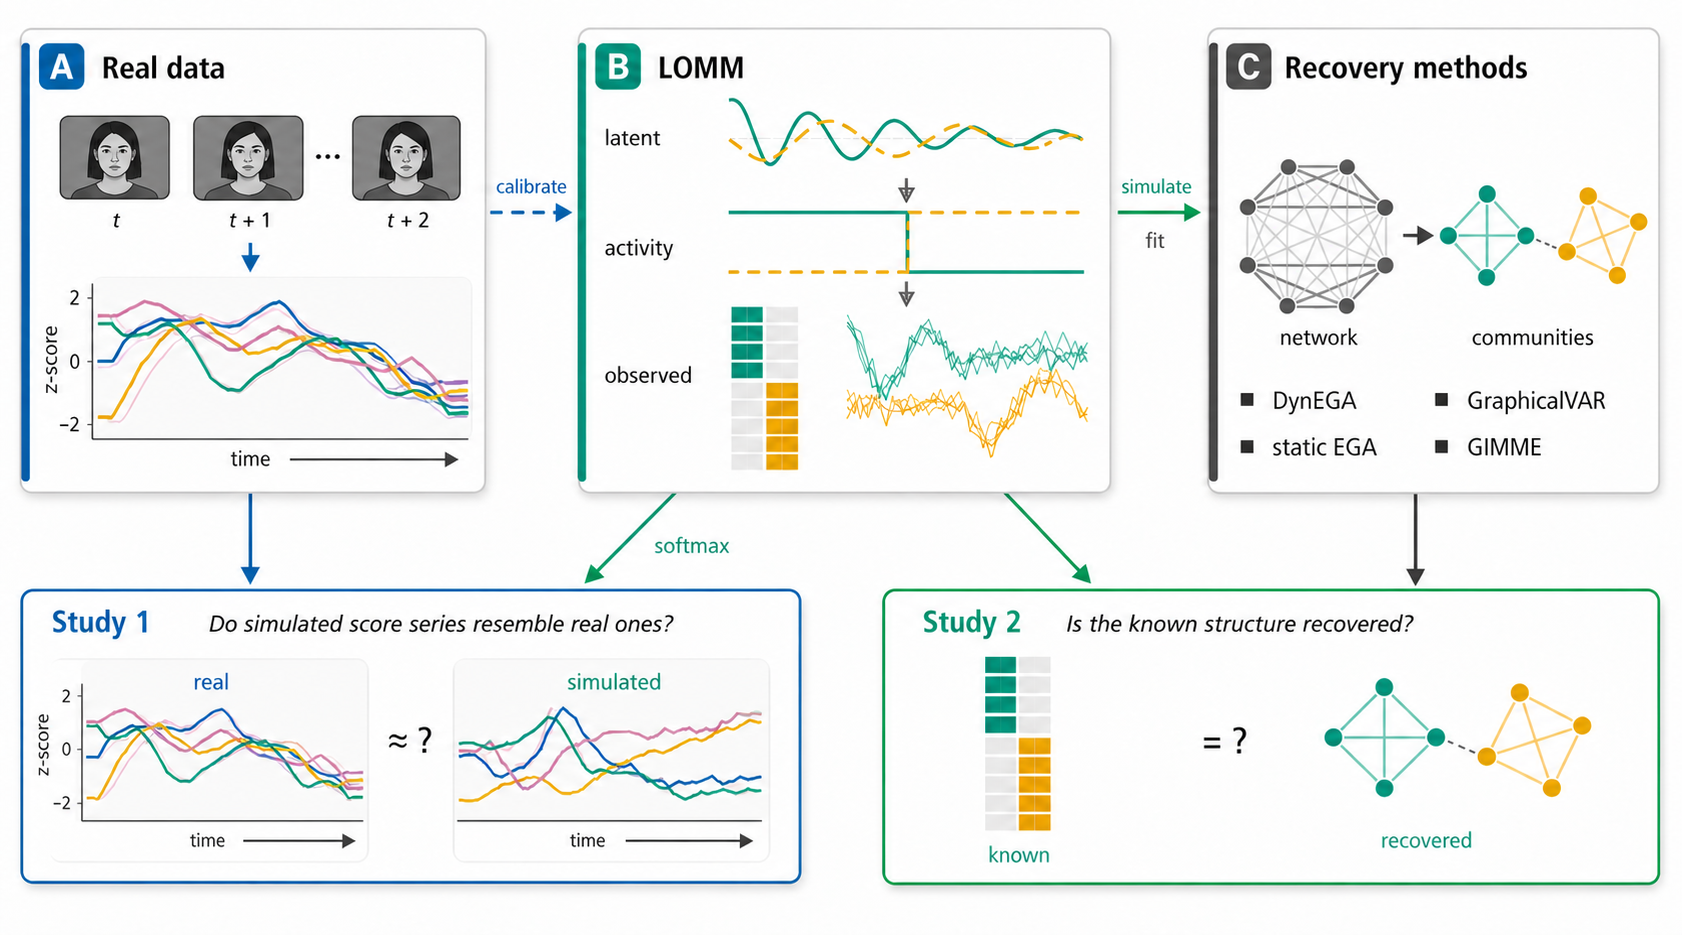
\includegraphics[width=0.98\linewidth,height=\textheight,keepaspectratio]{figures/lomm_pipeline_visual_abstract_nhb.png}

}

\caption{\label{fig-pipeline}Overview of the two studies. (A) Real data:
a classifier scores each sampled frame of an MAFW video, giving one
score series per label. (B) LOMM: latent oscillators, an activity
schedule that sets how strongly each is expressed at each observation,
and observed indicators with a known assignment to dimensions (colored
blocks). (C) Recovery methods: DynEGA, static EGA, GraphicalVAR, and
GIMME each estimate a network among the indicators and group them into
communities. Study 1 uses MAFW calibration videos to set the generator
and compares simulated score series with MAFW evaluation series. Study 2
fits the four methods to simulated indicators and compares the recovered
communities with the known assignment.}

\end{figure}%

\section{The Latent Oscillator Measurement
Model}\label{the-latent-oscillator-measurement-model}

Emotion labels can share broader psychological functions, including
engagement with desirable opportunities, defense against threats, and
attention to novel events (\citeproc{ref-bradley2009Orienting}{Bradley,
2009}; \citeproc{ref-lang2010Motivational}{Lang \& Bradley, 2010}).
These functions motivate an illustrative LOMM simulation with three
latent dimensions labeled approach-affiliation, threat-defense, and
orienting-novelty. Consider the threat-defense dimension: fear and
anxiety both concern responses to threat, although they involve
different defensive functions
(\citeproc{ref-mcnaughton2004Defense}{McNaughton \& Corr, 2004}). A
researcher could therefore specify fear, anxiety, worry, and
apprehension score channels as indicators of a shared threat-related
process. In the simulation, these channels covary as that process
changes over time, while each also contains measurement error. Other
channels measure the remaining two dimensions. The recovery task is to
identify the three dimensions and their indicator assignments. This
grouping is a theory-informed simulation hypothesis; whether empirical
classifier scores exhibit it requires separate investigation.

LOMM generates data in three layers (Figure~\ref{fig-lomm-process}). The
latent layer describes how each latent dimension changes over time. The
activity layer determines how strongly that dimension is expressed at
each observation. The observation layer creates multiple indicators with
prespecified loadings and measurement error. Keeping these layers
separate allows a researcher to change the dynamics, the expression
pattern, or the measurement quality while holding the other components
fixed.

\emph{Notation.} Suppose we have \(N\) video clips, each represented by
\(T\) sampled frames. Scoring each sampled frame produces one
multivariate observation. We index clips by \(i=1,\ldots,N\) and
observations within a clip by \(n=1,\ldots,T\). Observations occur at
times \(t_n=(n-1)\Delta\), where \(\Delta\) is the interval between
successive observations. Latent dimensions are indexed by
\(f=1,\ldots,m\). Continuous indicators are indexed by \(j=1,\ldots,p\);
in Study 2, \(p=mk\) with \(k\) indicators per dimension. Bounded scores
have \(J\) channels. Bold symbols are vectors or matrices.

For clip \(i\) and latent dimension \(f\), let \(x_{if}(t)\) denote the
latent level and \(\dot{x}_{if}(t)\) its rate of change. LOMM treats
each dimension as a linear second-order oscillator:

\begin{equation}
\ddot{x}_{if}(t)
=
\eta_f x_{if}(t)
+
\zeta_f\dot{x}_{if}(t)
+
q_{if,n},
\qquad t\in[t_n,t_{n+1}).
\label{eq:lomm-latent}
\end{equation}

Equation 1 is the damped linear oscillator used in research on
intraindividual dynamics (\citeproc{ref-boker2002Method}{Boker \&
Nesselroade, 2002}). Affective-dynamics models describe how emotional
states depart from and return toward a characteristic baseline. Damped
oscillator models represent this process through a tendency to return
toward baseline and a separate tendency for ongoing fluctuations to
diminish (\citeproc{ref-chow2005Thermostat}{Chow et al., 2005}). LOMM
uses these dynamics to generate latent expressive trajectories with
different patterns of persistence, recovery, and amplification.

The position-feedback parameter \(\eta_f\) determines how strongly a
deviation from baseline changes the direction of the trajectory. When
\(\eta_f<0\), values above baseline produce a downward acceleration and
values below baseline produce an upward acceleration. The
velocity-feedback parameter \(\zeta_f\) determines whether ongoing
changes are slowed or reinforced. Negative values oppose the current
direction of change and damp fluctuations; zero adds no damping;
positive values reinforce the change and amplify it. These parameters
describe the simulated dynamics; interpreting them as individual
differences in emotion regulation would require validation against
independent psychological measures. The term \(q_{if,n}\) is a random
acceleration input, drawn independently for each interval between
observations \(n\) and \(n+1\) and held constant within that interval;
it produces irregular peaks and reversals in the trajectory.

When both feedback parameters are negative, the process tends to settle
toward its baseline after a disturbance. It may approach the baseline
smoothly or move above and below it with progressively smaller swings.
New random inputs can keep these fluctuations going. Positive velocity
feedback instead reinforces ongoing changes and can produce increasingly
large swings. We include these growing trajectories to test whether the
methods can recover the specified dimensions when signal amplitudes
increase over a clip. Appendix C in the supplementary material reports
how large the simulated amplitudes become. These conditions are
evaluated over a fixed observation period; continued growth would
eventually become implausible for sustained expressive behavior.
Appendix A in the supplementary material gives the equations used to
calculate each successive latent state, explains which parameter
settings produce stable behavior, and describes how the starting values
are chosen.

The activity layer represents how strongly a latent process contributes
to the observed expression at a particular moment. Separating a process
from its expression is motivated by evidence that outward emotional
behavior can change without a corresponding change in reported
experience, as in expressive suppression
(\citeproc{ref-gross1993Suppression}{Gross \& Levenson, 1993}). In LOMM,
the nonnegative activity value \(a_{if,n}\) scales the latent signal:
\(\tilde{x}_{if,n}=a_{if,n}x_{if,n}\). Small values weaken its
contribution to the indicators, and larger values strengthen it. The
activity schedule is specified by the researcher and can represent
periods of weaker or stronger expression. It does not identify the
psychological mechanism producing those changes. This layer matters for
recovery because an abrupt change in activity can produce a large change
in the observed indicators even when the latent level remains
continuous.

The observation layer is a standard factor model:

\begin{equation}
\mathbf z_{in}
=
\boldsymbol\Lambda_i^{(z)}\tilde{\mathbf x}_{in}
+
\boldsymbol\varepsilon_{in}^{(z)},
\qquad
\boldsymbol\varepsilon_{in}^{(z)}\sim\mathcal N(\mathbf 0,\boldsymbol\Psi_i).
\label{eq:lomm-measurement}
\end{equation}

Row \(j\) of \(\boldsymbol\Lambda_i^{(z)}\) contains the loadings of
indicator \(j\) on the \(m\) latent dimensions, and
\(\boldsymbol\varepsilon_{in}^{(z)}\) is measurement error with
covariance \(\boldsymbol\Psi_i\). Appendix A in the supplementary
material gives the complete observation equations, including the
separate notation for continuous indicators and log-ratio coordinates
and the optional clip-specific baseline and scale terms.

\begin{figure}

\centering{

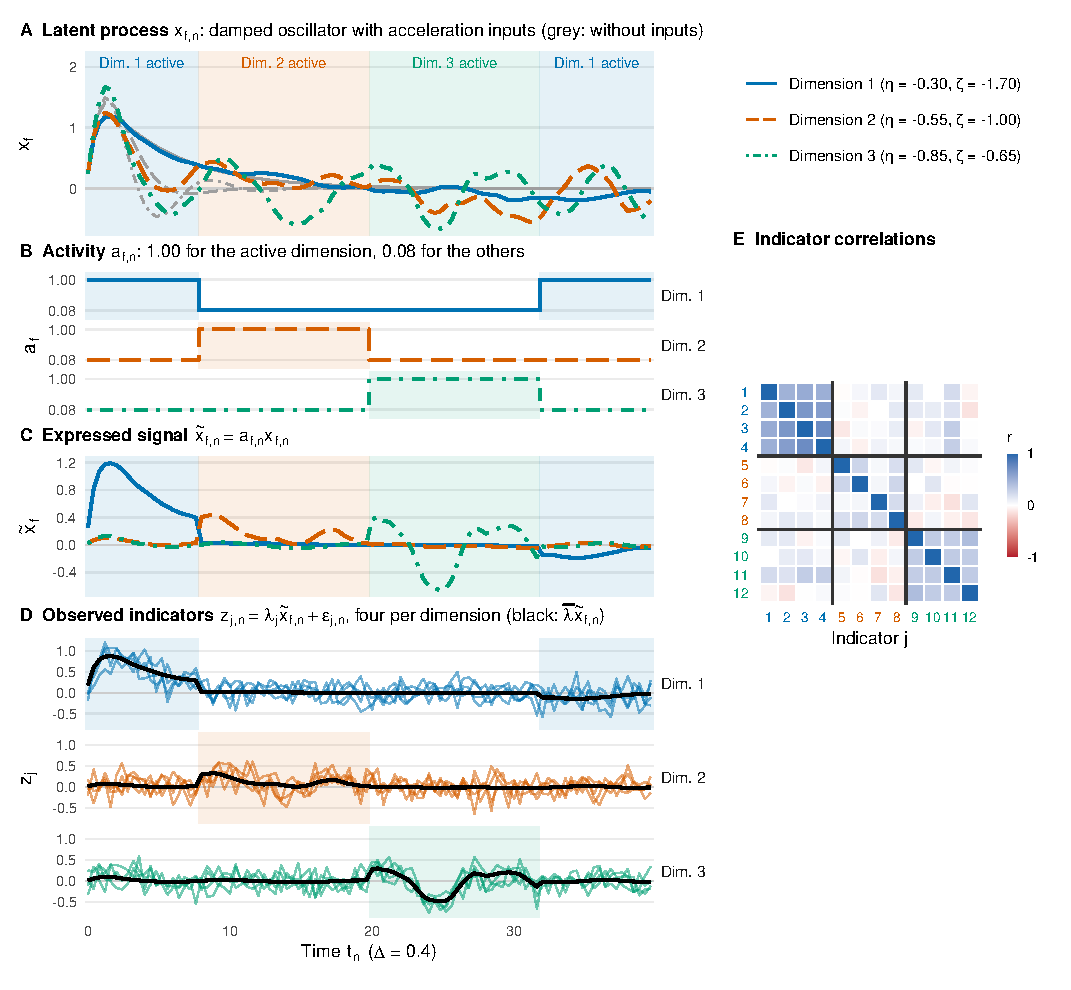
\includegraphics[width=0.98\linewidth,height=\textheight,keepaspectratio]{figures/lomm_process_overview.pdf}

}

\caption{\label{fig-lomm-process}One simulated LOMM clip with three
latent dimensions, \(T=100\) observations, and \(\Delta=0.4\). Each
column follows one dimension from the latent layer to the observed
indicators. (A) Latent trajectory; the oscillator parameters are given
in the column headers, and each dimension has its own initial state and
acceleration inputs. (B) Activity, 1.00 in the shaded active interval
and 0.08 otherwise. (C) Expressed signal, the product of the latent
level and the activity value, drawn over the latent level in grey. (D)
The four observed indicators of each dimension in shades from light to
dark, with primary loadings 0.65 to 0.85, secondary loadings of
\(\pm 0.30\) or \(\pm 0.35\) on another dimension for nine of the twelve
indicators, and residual SD 0.20. (E) Correlations among the twelve
indicators from this clip, ordered by dimension.}

\end{figure}%

Figure~\ref{fig-lomm-process} shows the three layers for one simulated
clip. In panel A the dimensions differ in their feedback parameters and
start from different states: dimension 1 rises to an early peak and
decays smoothly, dimension 2 starts in a trough and rebounds, and
dimension 3 oscillates faster and is driven mainly by its acceleration
inputs. Panel B shows the activity schedule, in which the dimensions
take turns being active. Panel C shows the product of the two layers. A
latent peak that falls inside an active interval is expressed at full
size; the same peak outside the interval is reduced to 8\% of its size
and is barely visible in the indicators. The steps at the boundaries of
the active intervals appear in the indicators although the latent level
remains continuous. Panel D shows the twelve indicators; each loads
mainly on its own dimension, and nine also carry a smaller loading on
another dimension. Panel E shows the correlation matrix among the twelve
indicators from this clip. The three diagonal blocks reflect the
indicator assignments, which is the structure that Study 2 asks the
methods to recover. The weaker correlations between blocks can reflect
both secondary loadings and sample covariation among the expressed
latent trajectories. The secondary loadings in this example are larger
than in the Study 2 cross-loading condition, which limits them to
\(\pm 0.10\).

LOMM can output two types of observed variables. The first is the vector
of continuous indicators \(\mathbf z_{in}\), used in the primary Study 2
designs; there, the factor structure that generated the data is defined
directly on the analyzed variables. The second is a vector of \(J\)
positive scores that sum to one, which matches the form of classifier
output and is used in Study 1. To produce bounded scores, LOMM maps the
latent dimensions to a \((J-1)\)-dimensional vector of log-ratio
coordinates and applies the softmax function. Because scores that sum to
one are compositional data, they are analyzed both as scores and in
log-ratio coordinates, which remove the sum constraint. A separate Study
2 condition applies the softmax directly to the \(p\) continuous
indicators and tests whether their original grouping is preserved.
Appendix A in the supplementary material gives the softmax, log-ratio,
and identification details.

In Study 1, MAFW calibration videos determine the LOMM observation-model
geometry and generator settings. The primary Study 2 design sets
between-clip baselines to zero and scales to one but lets loadings and
residual variances vary slightly across clips. Estimating oscillator,
activity, and measurement parameters from empirical data would require
the sign, scale, temperature, and frequency constraints stated in
Appendix A in the supplementary material.

\section{Study 1: Comparing Simulated and Real Score
Series}\label{study-1-comparing-simulated-and-real-score-series}

Study 1 examined whether LOMM, after calibration to MAFW, could generate
classifier-score series with statistical properties observed in MAFW
videos excluded from calibration. The analysis used 100 videos from
MAFW, a large multimodal database of facial-expression video recorded in
naturalistic settings (\citeproc{ref-liu_mafw_2022}{Liu et al., 2022}).
Frames were scored with the transforEmotion R package
(\citeproc{ref-tomasevic2026TransforEmotion}{Tomašević et al., 2026})
using OpenAI's CLIP ViT-Large/14 model (setting \texttt{oai-large}),
with up to 50 frames sampled per video. Eleven labels from the MAFW
label set served as text prompts: anger, disgust, fear, happiness,
neutral, sadness, surprise, contempt, anxiety, helplessness, and
disappointment. For each scored frame, the eleven classifier-score
channels sum to one.

Figure~\ref{fig-mafwvideo} shows the classifier-score series for one
MAFW video. Frames without a detected face have missing scores, so each
video was divided into segments of consecutive scored frames. The
analysis contains 3,557 observations in 188 segments. Videos contribute
16 to 50 scored observations, with a median of 35; segment lengths range
from 1 to 50 observations, with a median of 13.5. Appendix B in the
supplementary material gives the face-detection, score-validity,
missing-data, and sampling details.

\begin{figure}

\centering{

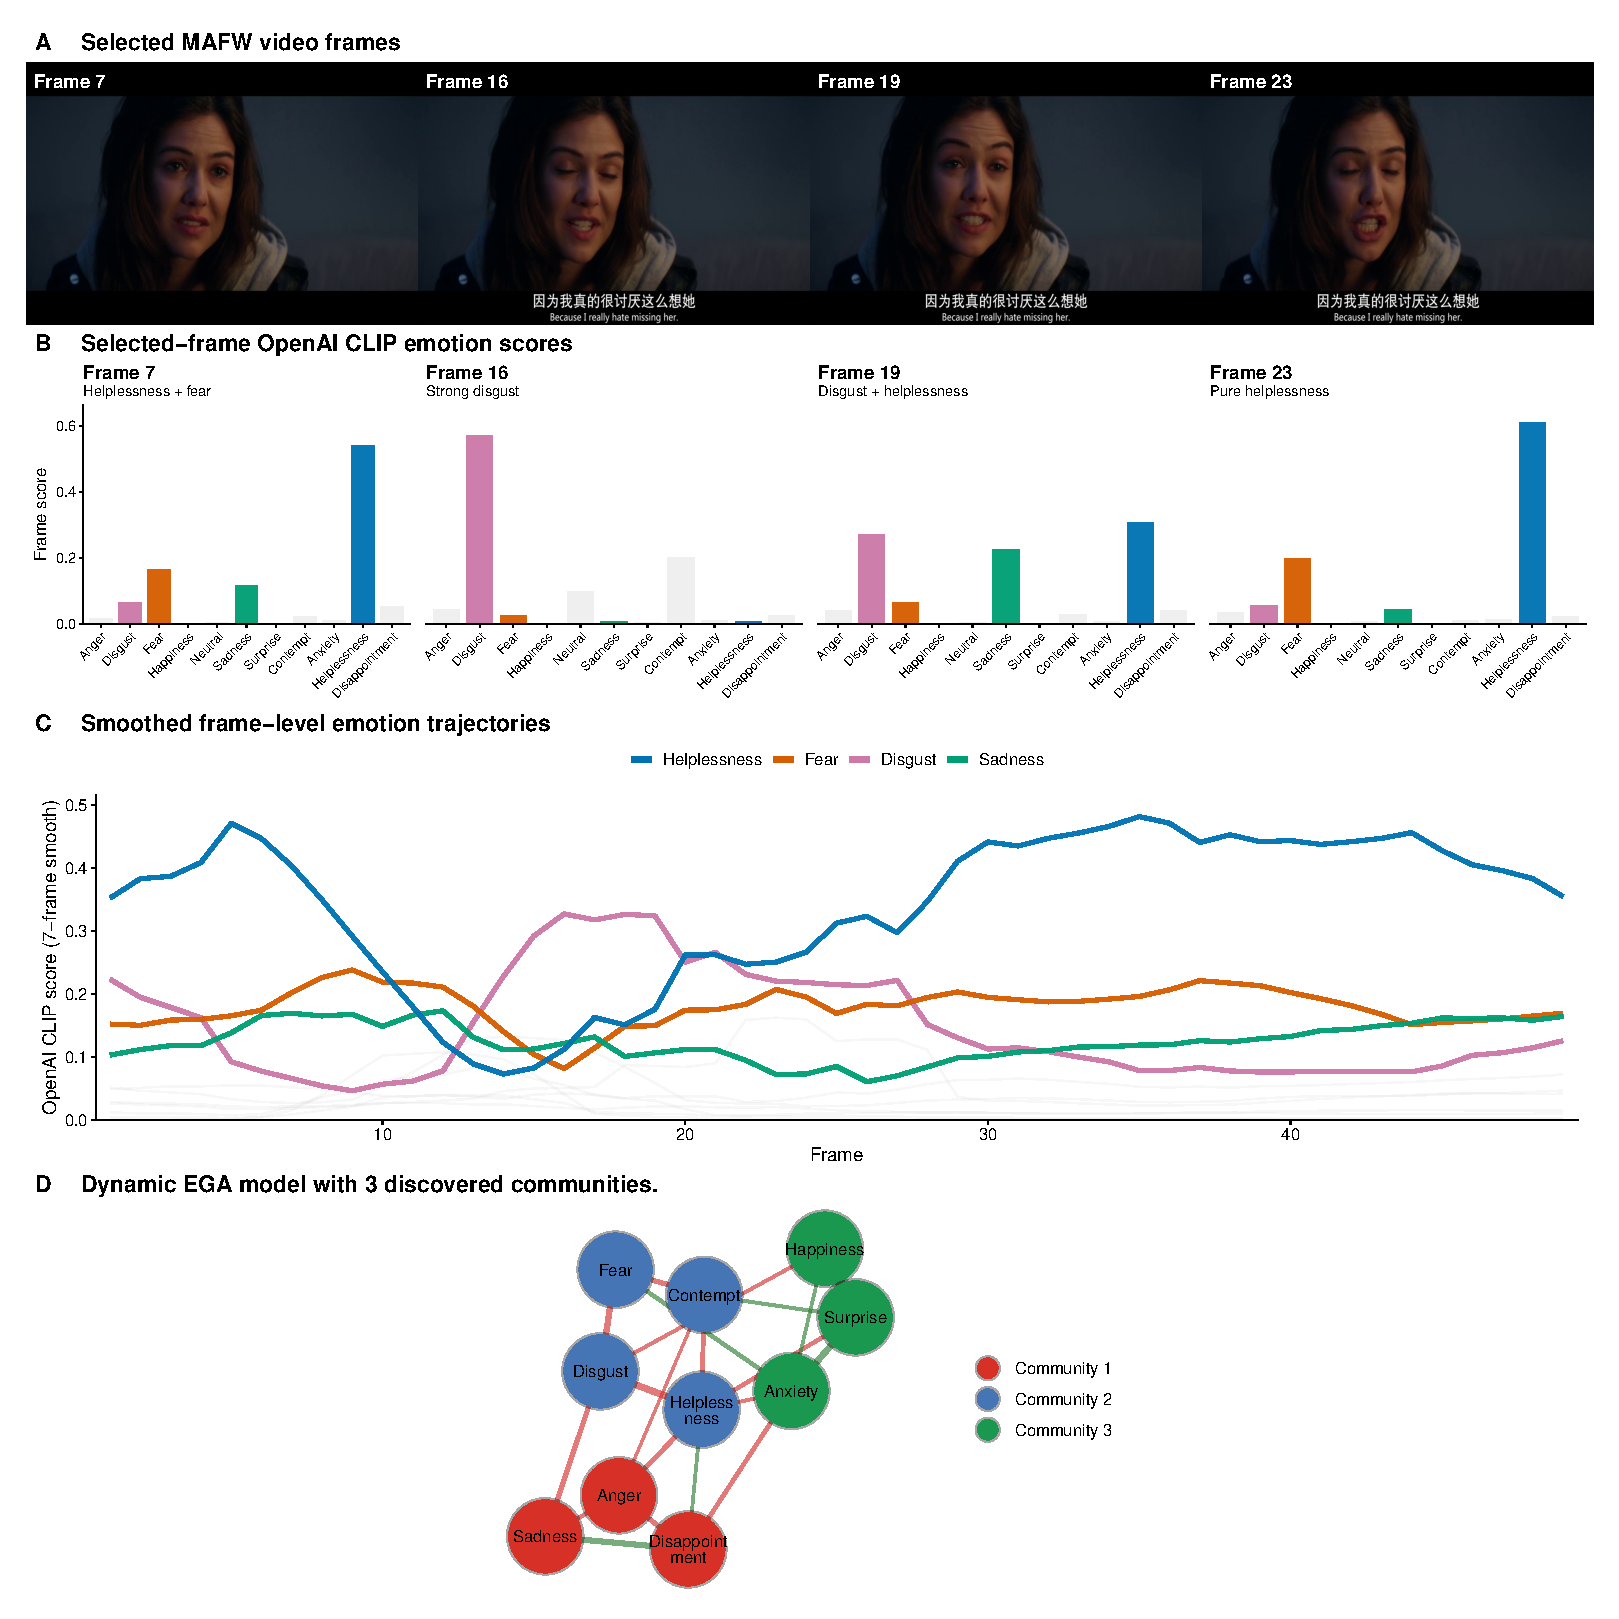
\includegraphics[width=0.98\linewidth,height=\textheight,keepaspectratio]{figures/mafw_video_dynega_example.pdf}

}

\caption{\label{fig-mafwvideo}Classifier-score series from one MAFW
video. Panel A shows four frames from the video, reproduced under the
MAFW research-use terms. Panel B shows the eleven classifier scores for
those frames. Panel C shows smoothed trajectories for the channels with
the highest mean scores. Scores were generated with transforEmotion
using OpenAI CLIP ViT-Large/14.}

\end{figure}%

We represented each MAFW and simulated series with a broad panel of
statistics covering location, dispersion, short-term change, temporal
persistence, temporal irregularity, and cross-channel dimensionality.
Eight statistics were computed within channel and video: median level;
interquartile range of levels; interquartile range of
observation-to-observation changes; lag-1 autocorrelation; and
run-length, sample, permutation, and spectral entropy. Their
channel-specific values were summarized by the median within each video.
Effective rank, robust level variance, and robust change variance
described all channels jointly. Each statistic was evaluated on the
classifier scores and a log-ratio representation, producing 22 features.
Channel statistics used centered log-ratios (CLR), and the three joint
statistics used isometric log-ratio (ILR) coordinates. The main analysis
combines the complete feature panel in the plausibility and coverage
measures. Appendix C in the supplementary material reports the
metric-specific comparisons.

We used four-fold cross-fitting. In each fold, 75 MAFW videos formed the
calibration set and 25 formed the evaluation set. The calibration set
determined the LOMM measurement geometry and the dynamic and measurement
parameters. LOMM then generated 100 datasets with the same observation
positions and uninterrupted segment boundaries as the evaluation videos.
We compared LOMM with a static logistic-normal generator calibrated from
the same 75 MAFW videos. The static generator retained the estimated
compositional structure, between-video heterogeneity, and observation
pattern while drawing observations independently over time. This
comparison estimates the gain associated with temporal generation beyond
static calibration.

For each fold, the MAFW reference comprised 1,000 comparisons between
two disjoint, category-stratified groups of 25 videos drawn from the 75
calibration videos. The 22 features were standardized using medians and
robust scales estimated from the calibration set. Series similarity was
measured by the root-mean-square Euclidean distance across these
standardized features. The similarity threshold was the 95th percentile
of the directional nearest-neighbor distances in the MAFW reference
comparisons. Plausibility is the proportion of simulated series whose
nearest MAFW evaluation series fell within this threshold. Coverage is
the proportion of MAFW evaluation series whose nearest simulation fell
within the threshold. Reported ranges are the 2.5th and 97.5th
percentiles across simulation or reference replicates. Appendix B in the
supplementary material gives the calibration, parameter selection,
metric, and reference-sampling procedures.

\section{Study 2: Recovery of Dimensionality and Indicator
Assignments}\label{study-2-recovery-of-dimensionality-and-indicator-assignments}

\emph{Data-generating conditions.} Study 2 asks whether four
network-based methods recover the number of latent dimensions and their
indicator assignments from LOMM-generated data. The primary comparison
applies all four methods to the same simulated datasets, including a
shorter-record condition. A larger factorial simulation evaluates DynEGA
across additional combinations of dimensionality, indicators per
dimension, and observation schedules. These analyses use continuous
indicators. Each dataset contains \(N\) clips with \(T\) observations
each and \(p=mk\) indicators. All clips share the same indicator
assignments and nominal measurement parameters, while allowing small
differences in measurement strength across clips. In these comparison
and factorial designs, each primary loading receives an independent
\(\operatorname{Unif}(-0.15,0.15)\) deviation, and each residual
variance receives an independent \(\operatorname{Unif}(-0.01,0.01)\)
deviation.

A latent dimension can be present in the generating model yet contribute
little observable variation during a short recording. Weak expression
can leave its indicators dominated by measurement error. When dimensions
alternate in prominence, each contributes strongly during only part of
the recording, and transitions can change the associations among
indicators. Increasing amplitudes can make later observations contribute
disproportionately to those associations. The six scenario families
examine recovery across these different patterns of expression while
keeping the indicator assignments fixed
(Table~\ref{tbl-scenario-words}). Families A and B represent weak and
strong expression with one dimension remaining dominant. Families C and
D allow the dominant dimension to change, with more rapid switching in
D. Families E and F introduce growing amplitudes, with either one
dominant dimension or switching dominance. These families combine
activity gains, switching schedules, and dynamic settings to represent
different recovery challenges. Appendix B in the supplementary material
gives the activity schedules and implementation details; Table B2 gives
the numerical oscillator parameters.

\begin{table}[H]

\caption{\label{tbl-scenario-words}The six Study 2 scenario families.
Numeric activity gains and dwell fractions are in Appendix B in the
supplementary material; oscillator parameters are in Table B2.}

\centering{

\begingroup\small\setlength{\tabcolsep}{6pt}

\begin{tabular}{cl}
\toprule
Code & Family\\
\midrule
A & Weak expression, one dominant dimension\\
B & Strong expression, one dominant dimension\\
C & Strong expression, switching dominant dimension\\
D & Strong expression, rapid switching\\
E & Amplifying dynamics, one dominant dimension\\
\addlinespace
F & Amplifying dynamics, switching dominant dimension\\
\bottomrule
\end{tabular}
\endgroup

}

\end{table}%

\emph{Recovery procedures.} Network methods provide a way to estimate
both the number of dimensions and the assignment of indicators to them.
In LOMM, indicators assigned to the same latent process share a changing
signal. Under suitable measurement conditions, this shared variation can
produce groups of strongly connected indicators in an estimated network.
Community detection can therefore identify candidate dimensions without
specifying their number in advance (\citeproc{ref-golino2017ega1}{H. F.
Golino \& Epskamp, 2017}). Study 2 examines whether this correspondence
survives changes in dynamics, expression strength, measurement error,
and observation length.

The four procedures construct networks from different aspects of the
same data: indicator levels, estimated changes, or residual associations
after temporal modeling (Table~\ref{tbl-method-roles}). Every method
receives the same simulated dataset. Each estimated structure is
converted to an undirected network by a prespecified rule, and a common
community-detection step identifies groups of indicators. Comparing
these groups with the generating assignments shows how well each
representation preserves the indicator partition, while retaining each
method's statistical model and data handling.

\begin{table}[H]

\caption{\label{tbl-method-roles}The four Study 2 methods, the structure
each supplies for the common grouping step, and its purpose in the
recovery comparison.}

\centering{

\begingroup\small\setlength{\tabcolsep}{3pt}

\begin{tabular}{lp{2.35in}p{2.35in}}
\toprule
Method & Structure used for grouping & Purpose in the recovery comparison\\
\midrule
DynEGA & Partial-correlation network of estimated changes & Assess recovery from coordinated changes in the indicators\\
Static EGA & Partial-correlation network of contemporaneous levels & Assess recovery from associations among indicator levels\\
GraphicalVAR & Contemporaneous residual partial-correlation network & Assess recovery from residual associations after modeling lagged relations\\
GIMME & Average residual-covariance network across clip-level fits & Assess recovery from residual associations after fitting each clip separately\\
\bottomrule
\end{tabular}
\endgroup

}

\end{table}%

DynEGA is included to test whether indicators driven by the same latent
process can be identified through their coordinated changes over time
(\citeproc{ref-glla2010}{Boker et al., 2010};
\citeproc{ref-golino2019investigating}{H. Golino et al., 2020};
\citeproc{ref-golino2020modeling}{H. Golino et al., 2022};
\citeproc{ref-golino2017ega1}{H. F. Golino \& Epskamp, 2017}). It
estimates first derivatives from time-delay embeddings, constructs a
regularized partial-correlation network among those derivatives, and
identifies communities as candidate dimensions. GraphicalVAR
(\citeproc{ref-epskampggm}{Epskamp et al., 2018};
\citeproc{ref-graphicalVAR2024}{Epskamp, 2024}) fits a multilevel vector
autoregression that separates lagged from contemporaneous relations; its
contemporaneous residual partial-correlation network is used for
grouping.

GIMME (\citeproc{ref-gates2012group}{Gates \& Molenaar, 2012};
\citeproc{ref-lane2019uncovering}{Lane et al., 2019}) fits a structural
vector autoregression to each clip separately. This allows the fitted
temporal and contemporaneous relationships to differ across clips.
Because the generating indicator assignments are shared across clips, we
examine whether that common grouping remains detectable in the residual
associations after these separate fits. Residual covariance matrices
from successful fits are averaged and submitted to the common
community-detection procedure. This adapts GIMME's usual use for
recovering individual-specific directed relationships to the recovery of
a shared indicator partition.

Static EGA estimates a regularized partial-correlation network from the
contemporaneous correlation matrix of indicator levels, ignoring the
observation order, and applies the same community-detection step. It
serves two purposes. Statistically, it shows how much of the grouping is
recoverable from contemporaneous levels alone; if most of it is, a
dynamic model cannot add much for this recovery target. Computationally,
it requires far less time than the dynamic methods. Comparing static EGA
with DynEGA and GraphicalVAR therefore shows whether modeling temporal
structure improves grouping enough to justify its computational cost in
these conditions.

\emph{Primary design and outcomes.} The primary design uses \(T=100\)
observations per clip and contains 21,600 datasets. It crosses the six
scenario families, \(m\in\{2,3\}\) dimensions, \(N\in\{50,100\}\) clips,
three loading levels (0.40, 0.60, 0.80), three residual standard
deviations (0.125, 0.25, 0.50), and 100 replications, with \(k=4\)
indicators per dimension. Every method receives the same dataset within
a condition and replication. The empirical videos motivate an additional
short-record condition. MAFW videos contain a median of 35 scored
observations, and uninterrupted segments have a median length of 13.5
observations. We therefore also evaluate recovery with \(T=25\), using
21,600 corresponding datasets. Louvain at resolution 1.0 is the primary
community-detection algorithm; Leiden and Walktrap were applied to the
same fitted networks as sensitivity analyses.

The primary outcome is the overall correct-dimension recovery rate: the
proportion of datasets in which the method returned a valid network and
the estimated number of dimensions equaled \(m\). A failed or timed-out
fit counts as an unsuccessful recovery. We also report the valid-output
rate and the correct-dimension rate among valid outputs, so that
computational feasibility and accuracy can be examined separately.
Assignment accuracy, the adjusted Rand index, and variation of
information compare the full estimated partition of indicators with the
true partition among valid outputs. Secondary diagnostics assess
alignment between the recovered groups and the activity-scaled latent
trajectories using best-match absolute trajectory correlation and
trajectory NRMSE. Appendix B in the supplementary material defines how
these diagnostics are constructed and matched.

\emph{Additional analyses.} Three additional analyses examine the limits
of the primary result. First, one-at-a-time sensitivity analyses start
from a reference condition (\(N=100\), \(T=100\), loading 0.60, residual
SD 0.25, common fixed initialization) and alter one design component at
a time by changing the initialization rule, smoothing activity
transitions, adding small cross-loadings, correlating residuals,
correlating acceleration inputs, or transforming the indicators to
bounded scores. The alternative initialization uses independent
stationary starts for stable dimensions and bounded independent starts
for amplifying dimensions. The bounded-score condition applies the
softmax function directly to the \(p\) continuous indicators and
analyzes either the \(p\) scores or their centered log-ratio (CLR)
components. Because the transformed scores must sum to one, the original
block structure among the \(p\) variables need not be preserved. Second,
a small analysis adds clip-specific baseline and scale differences, with
baselines constrained to the column space of the loading matrix so that
they add no structure outside the factor model. Third, an extended
factorial simulation of 518,400 datasets evaluates DynEGA alone over
additional numbers of dimensions, indicators per dimension, and
observation schedules. Appendix B in the supplementary material gives
the exact settings for every analysis.

\section{Results}\label{results}

\subsection{Study 1 Results: Similarity of Simulated and Real Score
Series}\label{study-1-results-similarity-of-simulated-and-real-score-series}

Figure~\ref{fig-mafw-clip-benchmark} compares the two generators with
the MAFW reference. LOMM achieved a median plausibility of 0.970 (95\%
simulation range {[}0.935, 0.990{]}) and coverage of 0.920 {[}0.900,
0.950{]}. The corresponding MAFW-to-MAFW reference values were 0.950
{[}0.910, 0.990{]} for both measures. The static logistic-normal
generator achieved plausibility of 0.510 {[}0.410, 0.590{]} and coverage
of 0.370 {[}0.290, 0.455{]}. LOMM therefore generated score series that
usually had a close MAFW counterpart and represented most MAFW
evaluation series, whereas static calibration alone covered
substantially less of the empirical variation.

\begin{figure}[H]

\centering{

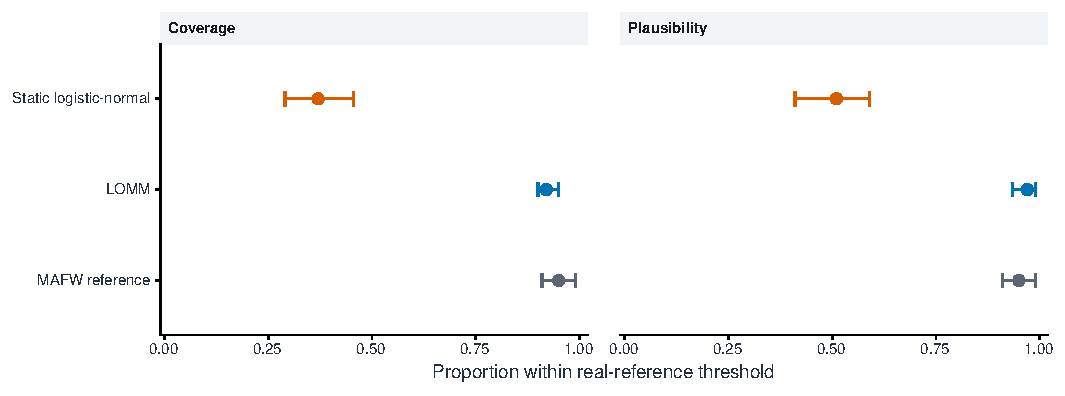
\includegraphics[width=0.95\linewidth,height=\textheight,keepaspectratio]{figures/figure4_mafw_clip_benchmark.pdf}

}

\caption{\label{fig-mafw-clip-benchmark}Cross-fitted similarity of LOMM
and static logistic-normal series to MAFW evaluation series. Points are
median proportions and bars are 2.5th and 97.5th percentiles across 100
generated datasets for each generator or 1,000 MAFW-to-MAFW reference
comparisons. Plausibility is the proportion of simulated series with a
nearest MAFW evaluation series within the fold-specific threshold.
Coverage is the proportion of MAFW evaluation series with a nearest
simulation within the same threshold. The threshold is the 95th
percentile of directional nearest-neighbor distances between disjoint
MAFW calibration samples. Higher values indicate closer agreement.}

\end{figure}%

Across the metric-specific comparisons, 14 of the 22 LOMM feature
discrepancies fell within the MAFW-to-MAFW reference range. Agreement
was strongest for dispersion, short-term change, temporal persistence,
and robust change variance. The clearest remaining differences concerned
sample entropy, which was higher in LOMM series, and spectral entropy,
which was lower. Appendix C in the supplementary material reports all
metric-specific results.

\subsection{Study 2 Results: Recovery of Dimensionality and Indicator
Assignments}\label{study-2-results-recovery-of-dimensionality-and-indicator-assignments}

Table~\ref{tbl-method-overall} reports the \(T=100\) results under
Louvain. The overall recovery rate requires both a valid network and the
correct number of dimensions, so every failure and timeout counts
against it. The last two columns report assignment accuracy among valid
outputs and median runtime.

\begingroup\scriptsize\setlength{\tabcolsep}{3pt}

\begin{longtable}[]{@{}
  >{\raggedright\arraybackslash}p{(\linewidth - 10\tabcolsep) * \real{0.1287}}
  >{\raggedleft\arraybackslash}p{(\linewidth - 10\tabcolsep) * \real{0.1287}}
  >{\raggedleft\arraybackslash}p{(\linewidth - 10\tabcolsep) * \real{0.1980}}
  >{\raggedleft\arraybackslash}p{(\linewidth - 10\tabcolsep) * \real{0.1683}}
  >{\raggedleft\arraybackslash}p{(\linewidth - 10\tabcolsep) * \real{0.1980}}
  >{\raggedleft\arraybackslash}p{(\linewidth - 10\tabcolsep) * \real{0.1782}}@{}}

\caption{\label{tbl-method-overall}Results for the primary \(T=100\)
design under Louvain. Assignment accuracy is computed among valid
network outputs. Runtime is the median, in seconds, among valid network
outputs and includes model fitting, network extraction, and community
detection.}

\tabularnewline

\toprule\noalign{}
\begin{minipage}[b]{\linewidth}\raggedright
Method
\end{minipage} & \begin{minipage}[b]{\linewidth}\raggedleft
Valid output
\end{minipage} & \begin{minipage}[b]{\linewidth}\raggedleft
Correct given valid
\end{minipage} & \begin{minipage}[b]{\linewidth}\raggedleft
Overall recovery
\end{minipage} & \begin{minipage}[b]{\linewidth}\raggedleft
Assignment accuracy
\end{minipage} & \begin{minipage}[b]{\linewidth}\raggedleft
Median runtime, s
\end{minipage} \\
\midrule\noalign{}
\endhead
\bottomrule\noalign{}
\endlastfoot
DynEGA & 1.000 & 0.939 & 0.939 & 0.965 & 3.69 \\
Static EGA & 0.997 & 0.887 & 0.884 & 0.922 & 2.15 \\
GraphicalVAR & 0.941 & 0.826 & 0.777 & 0.902 & 85.41 \\
GIMME & 0.224 & 0.783 & 0.176 & 0.877 & 518.16 \\

\end{longtable}

\endgroup

DynEGA returned a valid network for all 21,600 datasets and had the
highest overall recovery rate, 0.939. Static EGA followed at 0.884,
which shows that most of the grouping was recoverable from
contemporaneous indicator levels. GraphicalVAR reached 0.777. GIMME
recovered the correct dimension in 0.783 of its valid outputs but
returned a valid network for only 0.224 of datasets, so its overall
recovery was 0.176. Assignment accuracy among valid outputs was 0.965
for DynEGA, 0.922 for static EGA, 0.902 for GraphicalVAR, and 0.877 for
GIMME. Static EGA was about 40 times faster than GraphicalVAR and had
higher overall recovery and assignment accuracy for this target.
GraphicalVAR estimates a more complex model that includes lagged
effects; the comparison evaluates only whether that additional structure
improved recovery of the grouping under these conditions. Appendix C in
the supplementary material reports Monte Carlo standard errors,
bootstrap intervals, and the remaining partition diagnostics.

\begin{figure}[H]

\centering{

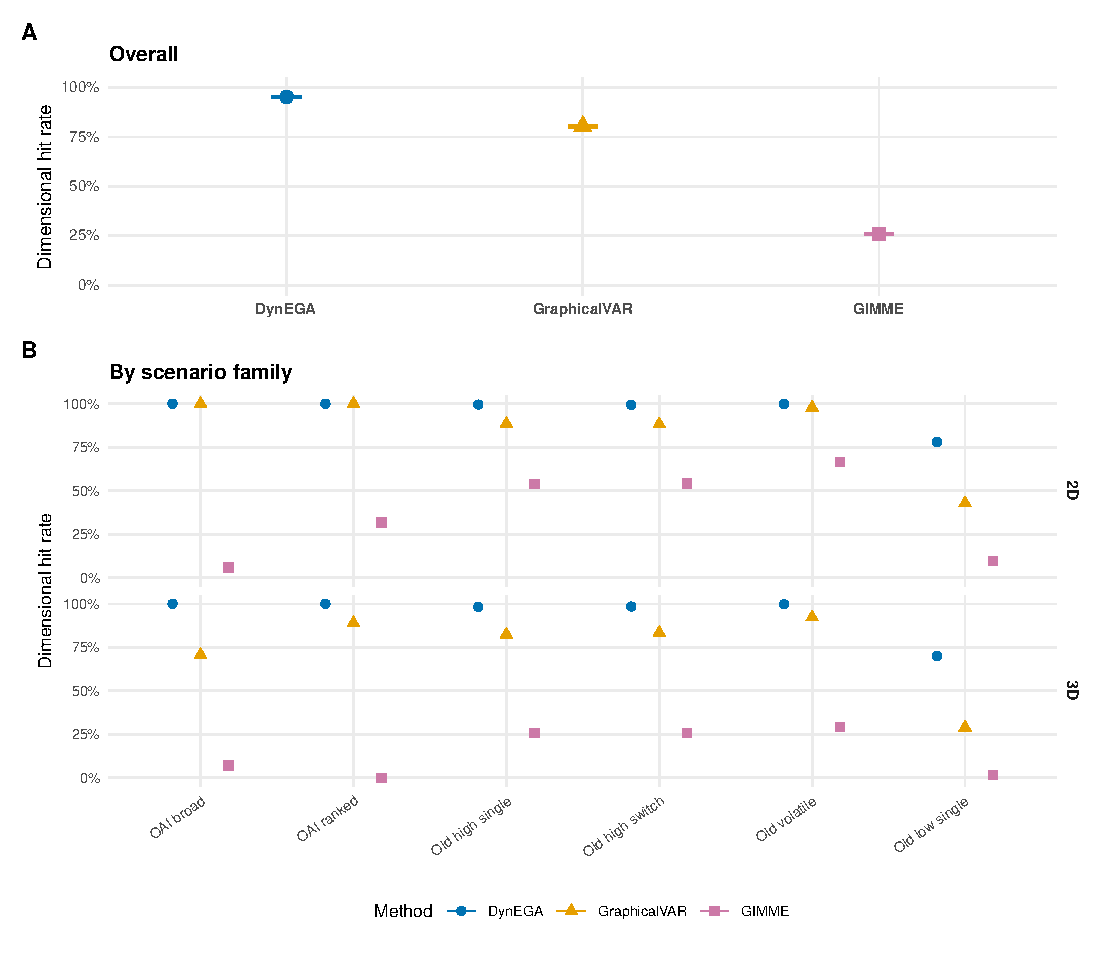
\includegraphics[width=0.98\linewidth,height=\textheight,keepaspectratio]{figures/figure5_dimension_recovery.pdf}

}

\caption{\label{fig-dimension-recovery}Overall correct-dimension
recovery under Louvain by scenario family (codes as in Table 1), method,
and observations per clip (\(T=100\), top; \(T=25\), bottom). A recovery
requires a valid network output and the correct number of dimensions.
Error bars are 95\% bootstrap intervals from resampling whole datasets.}

\end{figure}%

Recovery varied across scenario families and observations per clip
(Figure~\ref{fig-dimension-recovery}). DynEGA had the highest recovery
in most conditions. Static EGA's recovery was high because the block
structure was present in contemporaneous levels. GraphicalVAR's recovery
was lowest when expression was weak or measurement error was large.
GIMME's low overall rates mainly reflected missing valid outputs. In the
extended factorial simulation, DynEGA recovered the correct number of
dimensions in 93.7\% of 518,400 datasets and assigned 95.2\% of
indicators correctly; stronger loadings and smaller residual error
improved recovery. Leiden and Walktrap led to the same conclusions as
Louvain.

Secondary diagnostics assessed alignment between the recovered groups
and the activity-scaled latent trajectories. Among valid outputs with
the correct number of dimensions at \(T=100\), the best-match absolute
trajectory correlation and trajectory NRMSE were 0.760 and 0.602 for
DynEGA, 0.791 and 0.568 for GraphicalVAR, 0.606 and 0.898 for GIMME, and
0.787 and 0.563 for static EGA. GraphicalVAR and static EGA had higher
trajectory correlations and lower NRMSE than DynEGA, while DynEGA had
higher correlation and lower NRMSE than GIMME. These descriptive
comparisons condition on the outputs satisfying each method's
dimensional recovery criterion. Grouping recovery and trajectory
recovery are different targets, and neither ordering ranks the methods
in general. Appendix C in the supplementary material reports the
complete diagnostics.

\subsection{Robustness and Sensitivity
Analyses}\label{robustness-and-sensitivity-analyses}

\emph{Shorter records.} With \(T=25\), static EGA had the highest
overall recovery, 0.913, followed by DynEGA, 0.863, and GraphicalVAR,
0.770. Shortening the record slightly reduced DynEGA's recovery, left
GraphicalVAR's about the same, and increased static EGA's. At \(T=25\),
all 21,600 GIMME attempts ended in errors and none returned a valid
network; none was recorded as a timeout. Among outputs with the correct
number of dimensions, DynEGA's trajectory correlation was 0.848 and
NRMSE was 0.521; GraphicalVAR had the highest correlation and lowest
NRMSE, followed by DynEGA and static EGA (Appendix C in the
supplementary material).

\emph{Initial states.} In the reference condition of the one-at-a-time
analyses (\(N=100\), \(T=100\), loading 0.60, residual SD 0.25, common
fixed initialization), overall recovery was 0.993 for DynEGA, 0.912 for
static EGA, and 0.683 for GraphicalVAR. Replacing the common fixed
initialization with independent stationary starts for stable dimensions
and bounded independent starts for amplifying dimensions produced the
largest change among the sensitivity conditions: recovery fell to 0.838,
0.525, and 0.253, respectively. The common fixed initialization was
therefore optimistic relative to this alternative.

\emph{Other one-at-a-time changes.} Gradual activity transitions, small
cross-loadings, and correlated acceleration inputs changed recovery
little. A residual correlation of 0.10 between every pair of indicators
increased recovery for GraphicalVAR and static EGA. This result shows
that the particular residual pattern made the target grouping easier to
recover; it does not establish robustness to residual dependence more
generally.

\emph{Bounded scores.} Transforming the \(p\) indicators to scores that
sum to one changed the variables being analyzed and sharply reduced
recovery of the original grouping. DynEGA recovered the correct number
of dimensions in 0.333 of datasets analyzed as CLR components and 0.233
analyzed as raw scores; the corresponding rates were 0.333 and 0.167 for
static EGA and 0.087 and 0.002 for GraphicalVAR. The softmax
transformation and the accompanying projection onto the zero-sum
subspace did not preserve the structure among the original indicators.
For this reason, the Study 2 recovery results apply to continuous
indicators and are not extended to bounded scores of the kind analyzed
in Study 1.

\emph{Between-clip baseline and scale.} This analysis used stable
families A through D with independent stationary initial states. Its
reference recovery rates are lower than those in analyses using the
common fixed initialization. Adding clip-specific baseline and scale
changed DynEGA's recovery from 0.775 to 0.750, a paired difference of
\(-0.025\) (95\% interval \([-0.100,0.050]\)). Static EGA rose from
0.275 to 1.000: the added baselines lie in the column space of the
loadings, so they add between-clip variation that follows the intended
grouping. GraphicalVAR and GIMME were unchanged, but those estimates
rest on very few valid outputs; GraphicalVAR produced three correct
outputs among 80 datasets, and every three-dimensional GIMME fit timed
out.

\emph{Runtime and feasibility.} Median runtime among valid \(T=100\)
outputs was 2.15 s for static EGA, 3.69 s for DynEGA, 85.41 s for
GraphicalVAR, and 518.16 s for GIMME. GraphicalVAR timed out on 1,271 of
21,600 fits. GIMME produced 4,846 valid outputs, 14,477 timeouts, and
2,277 post-estimation errors. DynEGA returned a valid output for every
fit in the primary and extended designs. These runtimes are specific to
our implementation and hardware. Appendix C in the supplementary
material gives the full runtime, factorial, and community-detection
results.

\section{Discussion}\label{discussion}

LOMM separates three determinants of multivariate time-series structure:
the dynamics of latent processes, their expression over time, and their
measurement by observed indicators. This separation matters when
researchers use associations among classifier-score channels to infer
dimensional structure. A change in the recovered grouping may reflect a
different latent structure, weaker expression of an unchanged structure,
or properties of the measurement process. LOMM allows these
possibilities to be examined under controlled conditions by holding the
generating dimensions and indicator assignments fixed while varying
dynamics, activity, or measurement quality.

The two studies establish different parts of this contribution. Study 1
supports the statistical resemblance of calibrated bounded output to
short MAFW classifier-score series. Study 2 establishes recovery
performance for specified continuous-indicator models. The
initialization and bounded-score analyses show why those recovery
results require explicit conditions: changes in the starting states or
observation transformation can substantially change the recovered
structure.

Study 1 found that LOMM generated classifier-score series with high
plausibility and broad coverage relative to the MAFW reference. The
static logistic-normal generator preserved the calibrated score geometry
and between-video heterogeneity. It omitted temporal dependence and
performed substantially worse on both measures. In this comparison, LOMM
reproduced the joint statistical profile of the MAFW series more closely
than the calibrated static logistic-normal generator. The
metric-specific results also identify a concrete target for model
development: LOMM captured most measures of level, dispersion, change,
persistence, and cross-channel variation, while its entropy profile
remained less similar to MAFW.

Study 2 evaluated recovery of a known factor structure from continuous
indicators. DynEGA had the highest overall recovery in the primary
matched-method design and was feasible at the scale of the extended
factorial simulation, where it was the only method evaluated. Static EGA
showed that most of the grouping was recoverable from contemporaneous
levels; it exceeded GraphicalVAR in both dimensional recovery and
assignment accuracy while running in a median of 2.15 s rather than
85.41 s. For this grouping target and these conditions, GraphicalVAR's
additional lagged model did not improve recovery relative to static EGA.
GraphicalVAR answers additional questions about lagged relations, which
this comparison does not evaluate.

The trajectory diagnostics in Appendix C in the supplementary material
show that the ranking of methods depends on the recovery target.
DynEGA's advantage concerned recovery of the number of dimensions and
the indicator partition; alignment of recovered-group summaries with the
latent trajectories among valid outputs with the correct number of
dimensions produced a different ordering. The two targets should be
evaluated separately. All comparisons apply to the specific estimation,
network-conversion, and grouping procedures used here. GIMME's low
overall recovery mainly reflected its failure to return valid outputs
under a clip-level fitting procedure that differs from its usual use.

The most important qualification of the primary result concerns
initialization. Recovery was lower with independent stationary starts
for stable dimensions and bounded independent starts for amplifying
dimensions than with the common fixed initialization. The primary
initialization was therefore optimistic relative to this alternative.
Because this sensitivity changed cross-dimension and cross-clip
coherence together with the marginal initial-state distribution, it does
not isolate the effect of sharing alone. Gradual activity transitions,
small cross-loadings, and correlated acceleration inputs changed little.
The bounded-score condition set a clearer limit: the softmax
transformation changed the associations among the original indicators,
and neither the raw scores nor the CLR components preserved the original
grouping. The Study 2 recovery claims therefore apply to continuous
indicators.

\emph{Limitations.} Several limitations remain. The latent dimensions
are uncoupled. The amplifying families produce large amplitudes late in
the record and test recovery under those conditions only. The \(T=300\)
conditions also change the observation interval, so they do not isolate
the number of observations per clip. The GIMME residual-covariance
conversion was constructed for this comparison and differs from typical
idiographic use. Study 1 uses 100 short MAFW videos, one zero-shot
scoring pipeline, and one LOMM specification chosen during model
development on the same sample. LOMM is used here only as a generator
with prespecified parameters; estimating it from data would require the
identification constraints listed in Appendix A in the supplementary
material.

LOMM provides a generative basis for studying how latent dynamics,
changing expression, and measurement jointly shape multivariate
psychological time series. The present studies establish two initial
uses: generating bounded series that reproduce selected statistical
properties of video-derived emotion scores, and evaluating dimensional
recovery from continuous indicators with a known generating structure.
Together, they demonstrate how explicit assumptions about the generating
processes can support controlled evaluations of psychological
measurement. The bounded-score results also identify a central
methodological challenge: transforming latent signals into proportions
can change the observable structure on which dimensionality methods
rely.

A next step is to develop procedures for fitting LOMM to observed data
and recovering its dynamic, activity, and measurement parameters.
State-space and hierarchical continuous-time methods provide starting
points (\citeproc{ref-driver2018Hierarchical}{Driver \& Voelkle, 2018};
\citeproc{ref-ou2019Dynr}{Ou et al., 2019}), with parameter-recovery
studies needed to establish identification and estimation accuracy under
realistic sampling and measurement conditions. A particularly relevant
direction is the modeling of compositional time series, including gaze
allocation across areas of interest
(\citeproc{ref-facevicova2026Compositional}{Fačevicová et al., 2026}),
daily allocations of time among sleep and activity behaviors
(\citeproc{ref-le2022ActivitiesAffect}{Le et al., 2022}), and topic
proportions in repeated language samples
(\citeproc{ref-blei2006DynamicTopics}{Blei \& Lafferty, 2006}). In each
case, increasing one component's share necessarily reduces the combined
share of the others. LOMM's compositional observation layer offers a
basis for simulating such dependent trajectories while controlling the
latent processes that generate them. Extending this approach to
estimation would allow researchers to investigate which features of
psychological change remain identifiable when observations express
relative allocations. This would develop LOMM into a broader framework
for connecting theories of psychological dynamics with the constraints
of compositional measurement.

\newpage

\section{Declarations}\label{declarations}

\subsection{Funding}\label{funding}

The authors received no specific funding for this work.

\subsection{Competing interests}\label{competing-interests}

The authors declare that they have no competing interests.

\subsection{Ethics approval}\label{ethics-approval}

This study used simulations and secondary video data obtained under the
MAFW research-use terms. It involved no new recruitment, intervention,
or direct collection of human-participant data by the authors.

\subsection{Consent to participate}\label{consent-to-participate}

Not applicable.

\subsection{Consent for publication}\label{consent-for-publication}

The manuscript includes four still frames from MAFW solely to illustrate
the score-extraction procedure. The frames are cited to the dataset, and
no source video is redistributed. Their inclusion follows the dataset's
terms for limited reproduction in academic publications.

\subsection{Availability of data and
materials}\label{availability-of-data-and-materials}

The project GitHub repository at
\url{https://github.com/atomashevic/LOMM} contains the simulation
summary results, analysis-ready tables underlying the figures, and
aggregate MAFW-derived summaries used in the simulated-versus-real
comparison. Raw MAFW videos and frame-level classifier scores are not
redistributed. Access to MAFW is governed by the dataset provider, and
an end-to-end reanalysis of Study 1 requires approved access and local
generation of the classifier scores.

\subsection{Code availability}\label{code-availability}

Code for generating LOMM datasets, fitting the methods, reproducing the
statistical summaries, and regenerating the tables and figures is
available in the same GitHub repository. The repository also provides
the manuscript source and instructions for reproducing the analyses.

\subsection{Authors' contributions}\label{authors-contributions}

Aleksandar Tomašević contributed conceptualization, formal analysis,
methodology, resources, software, validation, visualization, writing the
original draft, and reviewing and editing the manuscript. Hudson Golino
contributed formal analysis, methodology, resources, software,
validation, visualization, writing the original draft, and reviewing and
editing the manuscript. Alexander P. Christensen contributed
methodology, software, writing the original draft, and reviewing and
editing the manuscript.

\section{Open Practices Statement}\label{open-practices-statement}

The study was not preregistered. The simulation and analysis code,
manuscript source, paper-facing tables, and aggregate MAFW-derived
summaries used in the simulated-versus-real comparison are available at
\url{https://github.com/atomashevic/LOMM}. Raw MAFW videos are
third-party materials, and the frame-level classifier scores are derived
from those restricted materials; neither is included.

\section{References}\label{references}

\begingroup
\setlength{\parindent}{-0.5in}
\setlength{\leftskip}{0.5in}

\phantomsection\label{refs}
\begin{CSLReferences}{1}{0}
\bibitem[\citeproctext]{ref-blei2006DynamicTopics}
Blei, D. M., \& Lafferty, J. D. (2006). Dynamic topic models.
\emph{Proceedings of the 23rd International Conference on Machine
Learning}, 113--120. \url{https://doi.org/10.1145/1143844.1143859}

\bibitem[\citeproctext]{ref-boker2015Adaptive}
Boker, S. M. (2015). Adaptive equilibrium regulation: {A} balancing act
in two timescales. \emph{Journal for Person-Oriented Research},
\emph{1}(1-2), 99--109. \url{https://doi.org/10.17505/jpor.2015.10}

\bibitem[\citeproctext]{ref-glla2010}
Boker, S. M., Deboek, P. R., Edler, C., \& Keel, P. (2010). Generalized
local linear approximation of derivatives from time series. In S. M.
Chow, E. Ferrer, \& F. Hsieh (Eds.), \emph{The notre dame series on
quantitative methodology. Statistical methods for modeling human
dynamics: An interdisciplinary dialogue} (pp. 161--178).
Routledge/Taylor \& Francis Group.

\bibitem[\citeproctext]{ref-boker2002Method}
Boker, S. M., \& Nesselroade, J. R. (2002). A {Method} for {Modeling}
the {Intrinsic Dynamics} of {Intraindividual Variability}: {Recovering}
the {Parameters} of {Simulated Oscillators} in {Multi-Wave Panel Data}.
\emph{Multivariate Behavioral Research}, \emph{37}(1), 127--160.
\url{https://doi.org/10.1207/S15327906MBR3701_06}

\bibitem[\citeproctext]{ref-bondielli2021CLIP}
Bondielli, A., \& Passaro, L. C. (2021). Leveraging {CLIP} for image
emotion recognition. \emph{Proceedings of the Fifth Workshop on Natural
Language for Artificial Intelligence, CEUR Workshop Proceedings},
\emph{3015}. \url{https://ceur-ws.org/Vol-3015/paper172.pdf}

\bibitem[\citeproctext]{ref-bradley2009Orienting}
Bradley, M. M. (2009). Natural selective attention: Orienting and
emotion. \emph{Psychophysiology}, \emph{46}(1), 1--11.
\url{https://doi.org/10.1111/j.1469-8986.2008.00702.x}

\bibitem[\citeproctext]{ref-chow2005Thermostat}
Chow, S.-M., Ram, N., Boker, S. M., Fujita, F., \& Clore, G. (2005).
Emotion as a thermostat: Representing emotion regulation using a damped
oscillator model. \emph{Emotion}, \emph{5}(2), 208--225.
\url{https://doi.org/10.1037/1528-3542.5.2.208}

\bibitem[\citeproctext]{ref-driver2018Hierarchical}
Driver, C. C., \& Voelkle, M. C. (2018). Hierarchical {Bayesian}
continuous time dynamic modeling. \emph{Psychological Methods},
\emph{23}(4), 774--799. \url{https://doi.org/10.1037/met0000168}

\bibitem[\citeproctext]{ref-graphicalVAR2024}
Epskamp, S. (2024). \emph{graphicalVAR: Graphical VAR for experience
sampling data}. \url{https://CRAN.R-project.org/package=graphicalVAR}

\bibitem[\citeproctext]{ref-epskampggm}
Epskamp, S., Waldorp, L. J., Mõttus, R., \& Borsboom, D. (2018). The
gaussian graphical model in cross-sectional and time-series data.
\emph{Multivariate Behavioral Research}, \emph{53}(4), 453--480.
\url{https://doi.org/10.1080/00273171.2018.1454823}

\bibitem[\citeproctext]{ref-facevicova2026Compositional}
Fačevicová, K., Vymazal, J., \& Popelka, S. (2026). Advancing eye
movement analysis through compositional modeling: A new perspective on
{Yarbus'} classic study. \emph{Behavior Research Methods}, \emph{58}(6),
173. \url{https://doi.org/10.3758/s13428-026-03054-5}

\bibitem[\citeproctext]{ref-foteinopoulou2023EmoCLIP}
Foteinopoulou, N. M., \& Patras, I. (2023). \emph{{EmoCLIP}: {A
Vision-Language Method} for {Zero-Shot Video Facial Expression
Recognition}} (arXiv:2310.16640). {arXiv}.
\url{https://doi.org/10.48550/arXiv.2310.16640}

\bibitem[\citeproctext]{ref-gates2012group}
Gates, K. M., \& Molenaar, P. C. M. (2012). Group search algorithm
recovers effective connectivity maps for individuals in homogeneous and
heterogeneous samples. \emph{NeuroImage}, \emph{63}(1), 310--319.
\url{https://doi.org/10.1016/j.neuroimage.2012.06.026}

\bibitem[\citeproctext]{ref-golino2017ega1}
Golino, H. F., \& Epskamp, S. (2017). Exploratory graph analysis: A new
approach for estimating the number of dimensions in psychological
research. \emph{PloS One}, \emph{12}(6), e0174035.
\url{https://doi.org/10.1371/journal.pone.0174035}

\bibitem[\citeproctext]{ref-golino2020modeling}
Golino, H., Christensen, A. P., Moulder, R., Kim, S., \& Boker, S. M.
(2022). Modeling latent topics in social media using dynamic exploratory
graph analysis: The case of the right-wing and left-wing trolls in the
2016 US elections. \emph{Psychometrika}, \emph{87}(1), 156--187.

\bibitem[\citeproctext]{ref-golino2019investigating}
Golino, H., Shi, D., Garrido, L. E., Christensen, A. P., Nieto, M. D.,
Sadana, R., Thiyagarajan, J. A., \& Martinez-Molina, A. (2020).
Investigating the performance of exploratory graph analysis and
traditional techniques to identify the number of latent factors: A
simulation and tutorial. \emph{Psychological Methods}, \emph{25}(3),
292--320. \url{https://doi.org/10.1037/met0000255}

\bibitem[\citeproctext]{ref-gross1993Suppression}
Gross, J. J., \& Levenson, R. W. (1993). Emotional suppression:
Physiology, self-report, and expressive behavior. \emph{Journal of
Personality and Social Psychology}, \emph{64}(6), 970--986.
\url{https://doi.org/10.1037/0022-3514.64.6.970}

\bibitem[\citeproctext]{ref-kankaanpaa2026multipleindicator}
Kankaanpää, R., Ron, J. de, Hoekstra, R. H. A., \& Bork, R. van. (2026).
Comparing multiple-indicator approaches to account for measurement error
in dynamic networks. \emph{Cognitive Therapy and Research}.
\url{https://doi.org/10.1007/s10608-026-10719-0}

\bibitem[\citeproctext]{ref-lane2019uncovering}
Lane, S. T., Gates, K. M., Pike, H. K., Beltz, A. M., \& Wright, A. G.
C. (2019). Uncovering general, shared, and unique temporal patterns in
ambulatory assessment data. \emph{Psychological Methods}, \emph{24}(1),
54--69. \url{https://doi.org/10.1037/met0000192}

\bibitem[\citeproctext]{ref-lang2010Motivational}
Lang, P. J., \& Bradley, M. M. (2010). Emotion and the motivational
brain. \emph{Biological Psychology}, \emph{84}(3), 437--450.
\url{https://doi.org/10.1016/j.biopsycho.2009.10.007}

\bibitem[\citeproctext]{ref-le2022ActivitiesAffect}
Le, F., Yap, Y., Tung, N. Y. C., Bei, B., \& Wiley, J. F. (2022). The
associations between daily activities and affect: A compositional
isotemporal substitution analysis. \emph{International Journal of
Behavioral Medicine}, \emph{29}(4), 456--468.
\url{https://doi.org/10.1007/s12529-021-10031-z}

\bibitem[\citeproctext]{ref-li2023CLIPER}
Li, H., Niu, H., Zhu, Z., \& Zhao, F. (2023). \emph{{CLIPER}: {A Unified
Vision-Language Framework} for {In-the-Wild Facial Expression
Recognition}} (arXiv:2303.00193). {arXiv}.
\url{https://doi.org/10.48550/arXiv.2303.00193}

\bibitem[\citeproctext]{ref-liu_mafw_2022}
Liu, Y., Dai, W., Feng, C., Wang, W., Yin, G., Zeng, J., \& Shan, S.
(2022). {MAFW}: A large-scale, multi-modal, compound affective database
for dynamic facial expression recognition in the wild. \emph{Proceedings
of the 30th ACM International Conference on Multimedia}, 24--32.
\url{https://doi.org/10.1145/3503161.3548190}

\bibitem[\citeproctext]{ref-mcnaughton2004Defense}
McNaughton, N., \& Corr, P. J. (2004). A two-dimensional neuropsychology
of defense: Fear/anxiety and defensive distance. \emph{Neuroscience and
Biobehavioral Reviews}, \emph{28}(3), 285--305.
\url{https://doi.org/10.1016/j.neubiorev.2004.03.005}

\bibitem[\citeproctext]{ref-mehu2015Emotion}
Mehu, M., \& Scherer, K. R. (2015). Emotion categories and dimensions in
the facial communication of affect: {An} integrated approach.
\emph{Emotion}, \emph{15}(6), 798--811.
\url{https://doi.org/10.1037/a0039416}

\bibitem[\citeproctext]{ref-nesselroade2002}
Nesselroade, J. R., McArdle, J. J., Aggen, S. H., \& Meyers, J. M.
(2002). Dynamic factor analysis models for representing process in
multivariate time-series. In D. S. Moskowitz \& S. L. Hershberger
(Eds.), \emph{Multivariate applications book series. Modeling
intraindividual variability with repeated measures data: Methods and
applications} (pp. 235-\/-265). Lawrence Erlbaum Associates Publishers.

\bibitem[\citeproctext]{ref-ou2019Dynr}
Ou, L., Hunter, M. D., \& Chow, S.-M. (2019). What's for {dynr}: A
package for linear and nonlinear dynamic modeling in {R}. \emph{The R
Journal}, \emph{11}(1), 91--111.
\url{https://doi.org/10.32614/RJ-2019-012}

\bibitem[\citeproctext]{ref-radford2021LearningTransferable}
Radford, A., Kim, J. W., Hallacy, C., Ramesh, A., Goh, G., Agarwal, S.,
Sastry, G., Askell, A., Mishkin, P., Clark, J., Krueger, G., \&
Sutskever, I. (2021). Learning transferable visual models from natural
language supervision. \emph{Proceedings of the 38th International
Conference on Machine Learning}, 8748--8763.

\bibitem[\citeproctext]{ref-russellCoreAffect2003}
Russell, J. A. (2003). Core affect and the psychological construction of
emotion. \emph{Psychological Review}, \emph{110}(1), 145--172.
\url{https://doi.org/10.1037/0033-295X.110.1.145}

\bibitem[\citeproctext]{ref-tomasevic2026TransforEmotion}
Tomašević, A., Golino, H., \& Christensen, A. (2026). {transforEmotion}:
An open-source {R} package for emotion analysis using transformer-based
generative {AI} models. \emph{Computational Communication Research},
\emph{8}(2), 1. \url{https://doi.org/10.5117/CCR2026.2.2.TOMA}

\bibitem[\citeproctext]{ref-nesselroade2008dfm}
Zhang, Z., Hamaker, E. L., \& Nesselroade, J. R. (2008). Comparisons of
four methods for estimating a dynamic factor model. \emph{Structural
Equation Modeling: A Multidisciplinary Journal}, \emph{15}(3), 377--402.
\url{https://doi.org/10.1080/10705510802154281}

\end{CSLReferences}

\endgroup




\end{document}
